\chapter{Introdução}
%%%%%%%%%%%%%%%%%%%%%%%%%%%%%%%%%%%%%%%%%%%%%%%%%%%%%%%%%%%%%%%%
As balanças foram criadas por necessidade durante o desenvolvimento de comercio na antiguidade, os produtos que não recorriam a contagem por unidades, tais como objetos irregulares por exemplo o ouro tinham de se quantificar seu valor, e a forma de medir sua massa tornou-se numa variável de medição para troca de bens.\\
\\
A relíquia mais antiga de uma balança de medir massa foi descoberto na vila de \textit{Indus River}, perto do conhecido por hoje de Pakistão, e estima-se ser por volta de 2000 B.C.\\
Estas primeiras balanças eram alavancas em equilíbrio $[ \; F_{1} \times b_{1c} = F_{2} \times b_{2c} \; ]$, onde nos extremos eram colocados cestos e se colocava os pesos, este estava centrado no seu centro de massa, assim se os pesos nos dois cestos serem iguais fica em equilíbrio (horizontal), era um sistema de comparar com pesos fixos estabelecidos como norma (\textit{contra-pesos}).
\\
\begin{minipage}[!b]{0.45\linewidth}
	\begin{figure}[H]
		\centering
		\includegraphics[height=7cm]{./image/PESTA/general/balanca_1.jpg}
		\caption{Balança medieval}
		\label{balanca_1}
	\end{figure}
\end{minipage}
\hspace{2.2cm}
\begin{minipage}[!b]{0.45\linewidth}
	\begin{figure}[H]
		\centering
		\includegraphics[height=7cm]{./image/PESTA/general/balanca_4.jpg}
		\caption{Balança}
		%\caption{Balança moderna \cite{book-7}}
		\label{balanca_4}
	\end{figure}
\end{minipage}
\newline
\newline
\newline
Este sistema pode ter uma boa precisão, mas também pode facilmente ser adulterado.
\\
\\
Os métodos de medir a massa de objetos não conheceu nenhumas melhorias tecnológicas relevantes até a era industrial. Só nos fins do século \textit{XVIII} é que o meio de medir a massa de objetos não dependia de \textbf{contra-pesos}. As balanças por molas foi inventado por \textbf{\textit{Richard Salter}}, um fabricante de balanças por volta dos anos de 1770 na Inglaterra.\\
\begin{figure}[H]
	\centering
	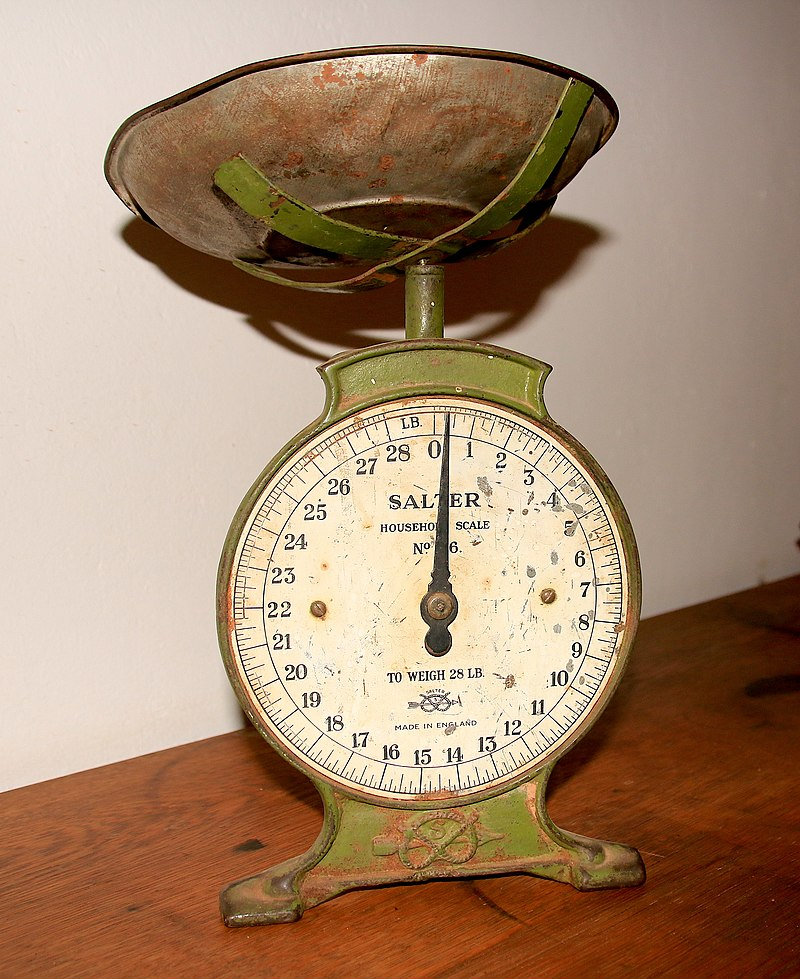
\includegraphics[height=7cm]{./image/PESTA/general/Weigh_Scale_Salter_1.jpg}
	\caption{Balança de Salter}
	\label{Weigh_Scale_Salter_1}
\end{figure}
A balança por mola, como o nome implica, mede a pressão (ou sua tensão) exercido sobre a mola para determinar a massa do objeto. Este tipo de balanças ainda são muito comum nos dias de hoje por serem bastante económicas de fabricar, mas não tem tanta precisão como as eletrónicas desenvolvidas e aperfeiçoadas durante o século \textit{XX}.
\newline
\newline
\begin{minipage}[!b]{\linewidth}
	\begin{figure}[H]
		\captionsetup{justification=raggedright,singlelinecheck=false}
		\flushleft
		\includegraphics[height=7cm]{./image/PESTA/general/Public_Body_Scales_1.jpg}
		\hspace{.8cm}
		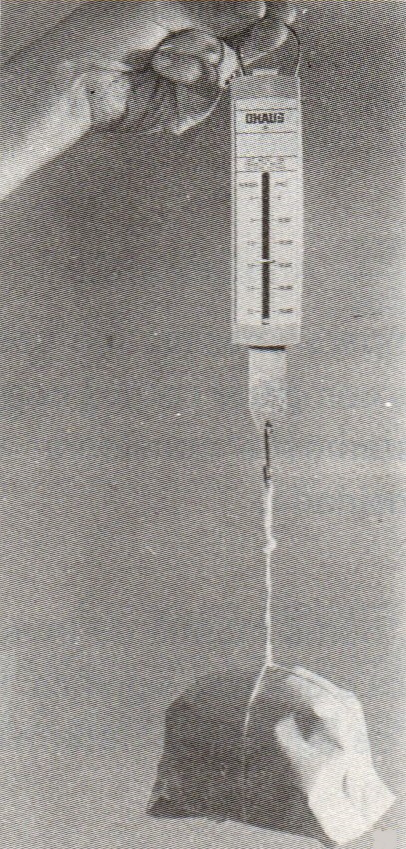
\includegraphics[height=7cm]{./image/PESTA/general/Balanca_Mola_1.jpg}
		\caption{Balanças de Mola}
		\label{Balanca_Mola_1}
	\end{figure}
\end{minipage}
\newpage
As balanças eletrónicas mais modernas utilizam resistências elétricas em materiais permeáveis e fazer passar uma corrente elétrica na qual é possível detetar a variação de condutividade das resistências em que é proporcional a pressão exercida sobre esse material, podendo dai se deduzir o peso dos objetos que se encontrem na balança.
\begin{figure}[H]
	\centering
	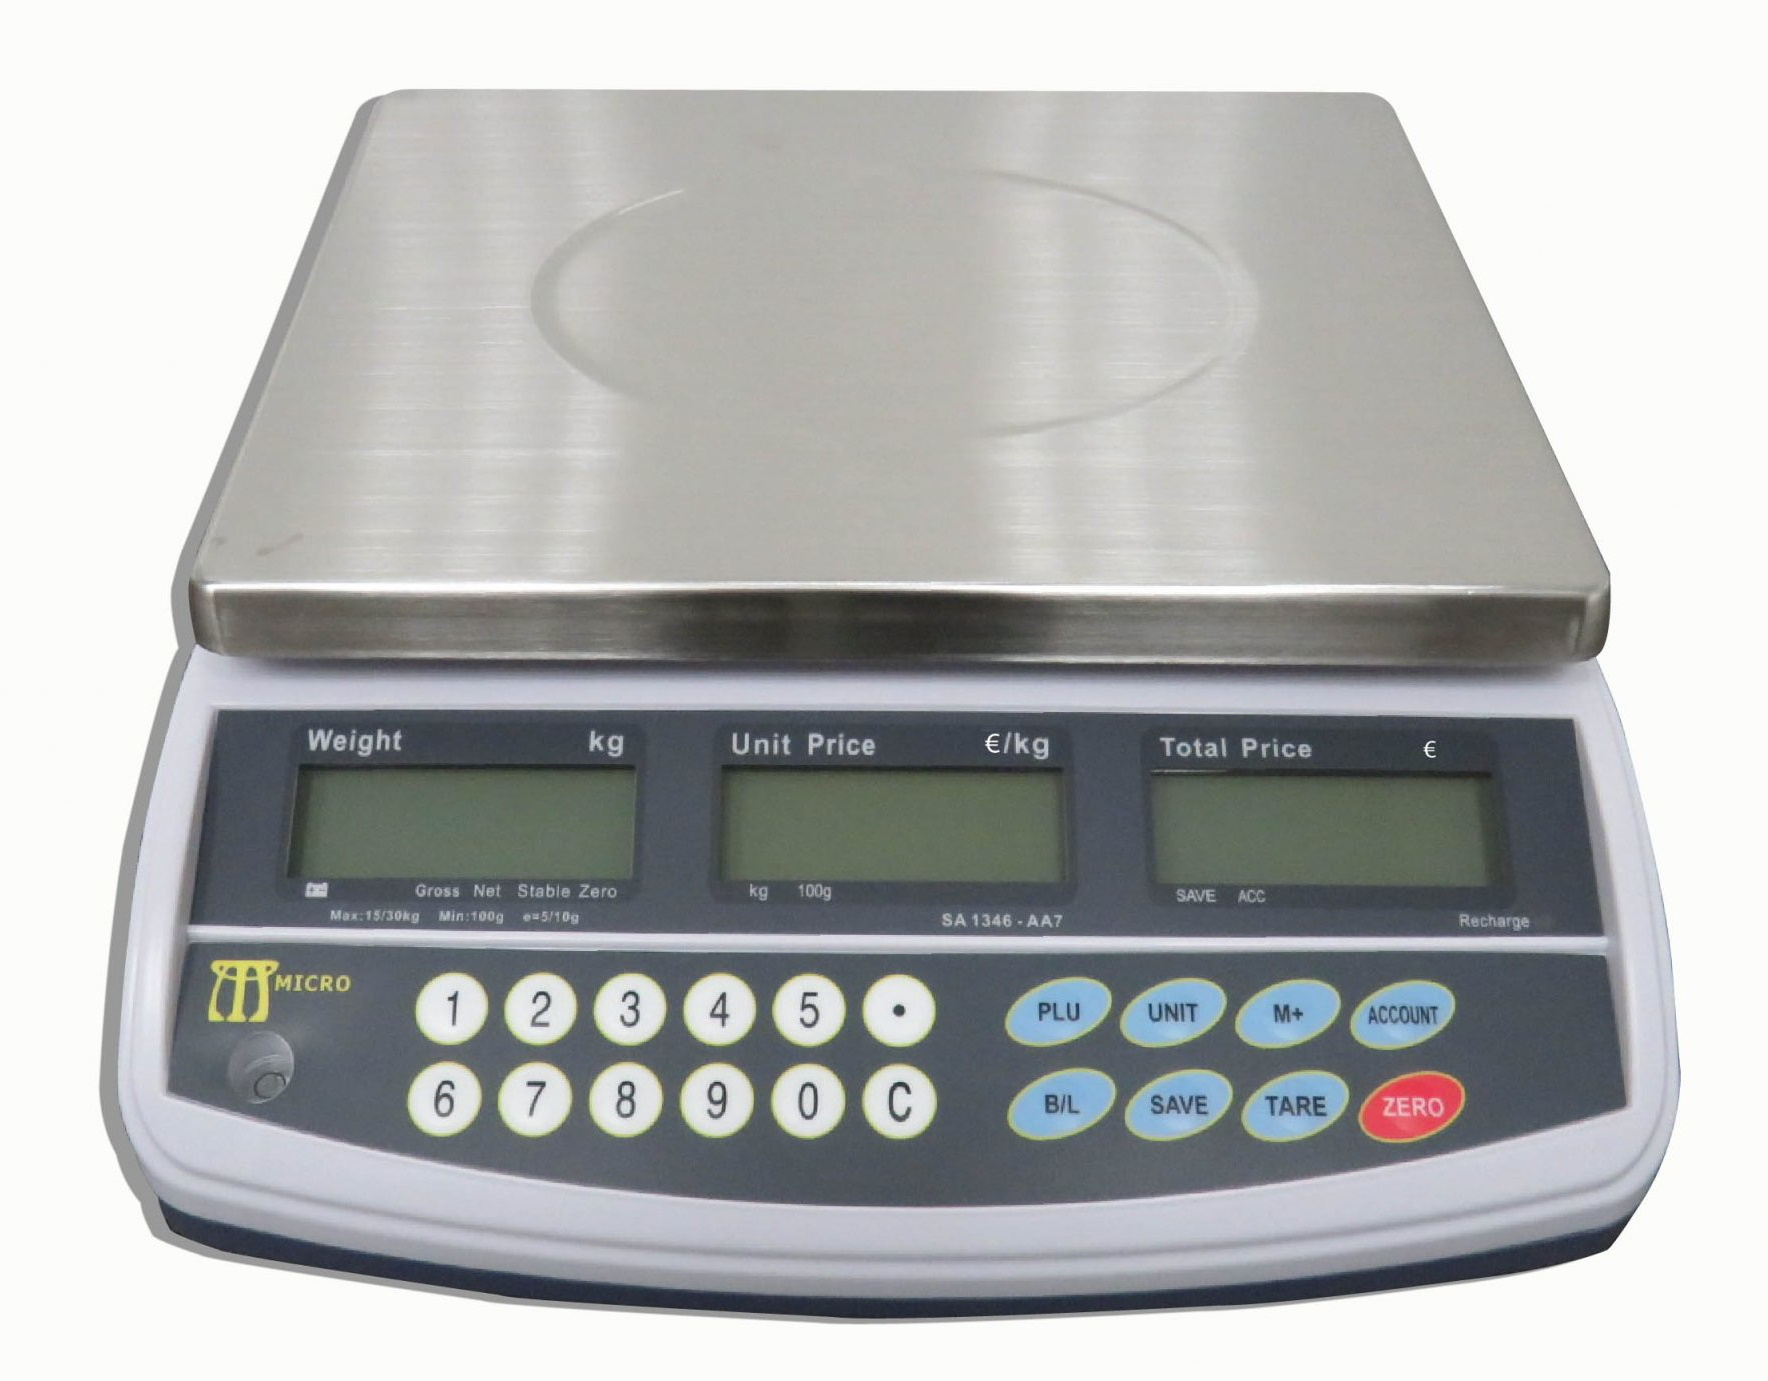
\includegraphics[height=7cm]{./image/PESTA/general/Scale_1.jpg}
	\caption{Balança eletrónica}
	\label{Sale}
\end{figure}
O que vai ser utilizado para o projeto vai ser um célula de peso que seque o principio acima mencionado, estes sensores tem quatro \textit{\textbf{strain gauges}} ligadas em ponte \textit{wheatstone} que vão detetar a distorção do material ou seja a célula de peso e gerar um sinal em tensão proporcional a força exercida. Seque o mesmo principio de uma mola $ [ \; K = \frac{\Delta l}{F} \; ] $.
\\
\\
Também há outros tipos de células de peso tais como as pneumáticas e hidráulicas que convertem a pressão num sinal elétrico que é proporcional a força nela exercida $ [ \; P = \frac{F}{A} \; ] $. As células de peso capacitivas são outro exemplo de como obter um sinal proporcional a força imposta como carga, neste caso é medido sua capacidade pelo afastamento ou aproximação dos pratos dos elétrodos $ [ \; C = \varepsilon_{0} \; \varepsilon_{r} \; \frac{A}{d} \; ] $.
\\
\\
Pode-se dizer que em todos os casos determina-se a força resultante através do deslocamento no espaço.\\
\\
\section*{Sensor}

Piezoresistivity derives its name from the Greek word piezin, meaning “to press.” It is an effect exhibited by various materials that exhibit a change in resistivity due to an applied pressure. The effect was first discovered by Lord Kelvin in 1856, who noted that the resistance of copper and iron wires increased when in tension. He also observed that iron wires showed a larger change in resistance than those made of copper. The first application of the piezoresistive effect did not appear until the 1930s, some 75 years after Lord Kelvin’s discovery. Rather than using metal wires, these so-called strain gauges are generally made from a thin metal foil mounted on a backing film, which can be glued onto a surface. A typical metal foil strain gauge is depicted in Figure 5.1. \cite{book-9}
\begin{figure}[H]
	\centering
	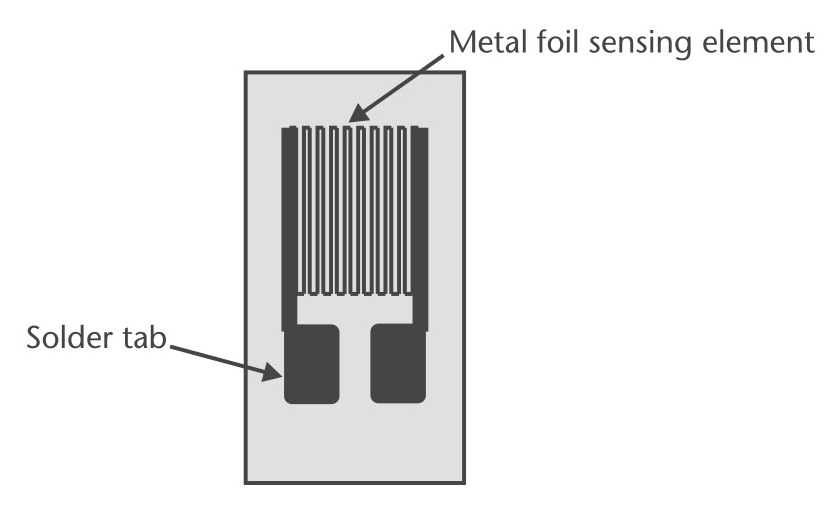
\includegraphics[height=5cm]{./image/PESTA/general/strain_gauge_1.jpg}
	\caption{Metal foil strain gauge \cite{book-9}}
	\label{strain_gauge_1}
\end{figure}

\section*{Amplificador}
Amplification is usually a fundamental requirement, as most sensors tend to
produce signal levels that are significantly lower than those used in the digital processor. Resistive sensors in a bridge configuration often require an instrumenta-tion amplifier; piezoelectric devices may need a charge amplifier. If possible, it is advantageous to have the gain as close as possible to the sensing element. In situations where a high gain is required, there can often be implications for han-dling any adverse effects such as noise. In terms of chip layout, the sharp transients associated with digital signals need to be kept well away from the front-end analog circuitry. \cite{book-9}

\section*{Informação}
Data conversion is the transition region between the continuous (real-world)
signals and the discrete signals associated with the digital processor. Typically, this	stage comprises an analog-to-digital converter (ADC). Inputs from other sensors (monitoring) can be fed into the data conversion subsystem and may be used to implement compensation, say for temperature. Note that such signals may also require amplification before data conversion. Resonant sensors, whose signals are in the frequency domain, do not need a data conversion stage as their outputs can often be fed directly into the digital system. The digital processing element mainly concerns the software processes within the smart sensor. These may be simple routines such as those required for imple-menting sensor compensation (linearization, cross-sensitivity, offset), or they may be more sophisticated techniques such as pattern recognition methods (such as neu- ral networks) for sensor array devices.\cite{book-9}
\\
\\
The data communications element deals with the routines necessary for pass-
ing and receiving data and control signals to the sensor bus. It is often the case that the smart sensor is a single device within a multisensor system. Individual sensors can communicate with each other in addition to the host system. There are many examples of commercial protocols that are used in smart sensor systems, but we will not go into detail here. It is sufficient to be aware that the smart sensor will often have to deal with situations such as requests for data, calibration signals, error checking, and message identification. Of course, it is feasible in some applica-
tions that the data communications may simply be a unit that provides an analog voltage or current signal. \cite{book-9}
\\
\\
The control processor often takes the form of a microprocessor. It is generally the central component within the smart sensor and is connected to most of the other elements, as we have already seen. The software routines are implemented within the processor and these will be stored within the memory unit. The control processor may also issue requests for self-test routines or set the gain of the amplifier. \cite{book-9}

%%%%%%%%%%%%%%%%%%%%%%%%%%%%%%%%%%%%%%%%%%%%%%%%%%%%%%%%%%%%%%%%
